%\section {Preventivo}
\section {Preventivo}
	\subsection {Introduzione}
    In questa sezione viene descritta la suddivisione del lavoro in vari \glo{Periodo}{periodi} e l'assegnazione ai membri del \glo{Gruppo}{gruppo} in base ai ruoli ricoperti. Verrà posta particolare attenzione all'aspetto economico.
    Verranno utilizzate le seguenti abbreviazioni:
   		\begin{itemize}
   		\item{\textbf{Re}}: \responsabilediprogetto;
     	\item{\textbf{Am}}: \amministratore;
     	\item{\textbf{At}}: \analista;
     	\item{\textbf{Pj}}: \progettista;
     	\item{\textbf{Pr}}: \programmatore;
     	\item{\textbf{Ve}}: \verificatore;
     	\item{\textbf{Tot}}: totale.
   		\end{itemize}

\newpage
	\subsection {Dettaglio periodi}
		\subsubsection {Periodo: An - Analisi}
			\paragraph{Preventivo orario}
%-----------------------------------------------------------------
							\begin{table}[H] \begin{center} \begin{tabular}{llllllll}
							\toprule
							\textbf{Nominativo}	&	\textbf{Re}	&	\textbf{Am}	&	\textbf{At}	&	\textbf{Pj}	&	\textbf{Pr}	&	\textbf{Ve}	&	\textbf{Tot}\\
							\midrule
							Brutesco	&	-	&	-	&	12	&	-	&	-	&	12	&	24	 \\
							Damo		&	-	&	9	&	15	&	-	&	-	&	-	&	24	 \\
							De Gaspari	&	-	&	-	&	12	&	-	&	-	&	12	&	24	 \\
							Gottardo	&	14	&	-	&	10	&	-	&	-	&	-	&	24	 \\
							Pasqualini	&	-	&	-	&	12	&	-	&	-	&	12	&	24	 \\
							Petenazzi	&	7	&	-	&	17	&	-	&	-	&	-	&	24	 \\
							Prete		&	-	&	10	&	14	&	-	&	-	&	-	&	24	 \\
							\midrule
							Tot. in ore	&	21	&	19	&	92	&	0	&	0	&	36	&	168	 \\

							\bottomrule
							\end{tabular} \end{center} \caption{Prospetto orario - \glo{Periodo}{Periodo}:
							An
							}\label{tab:h_An} \end{table}

								\begin{figure}[H]  \centering  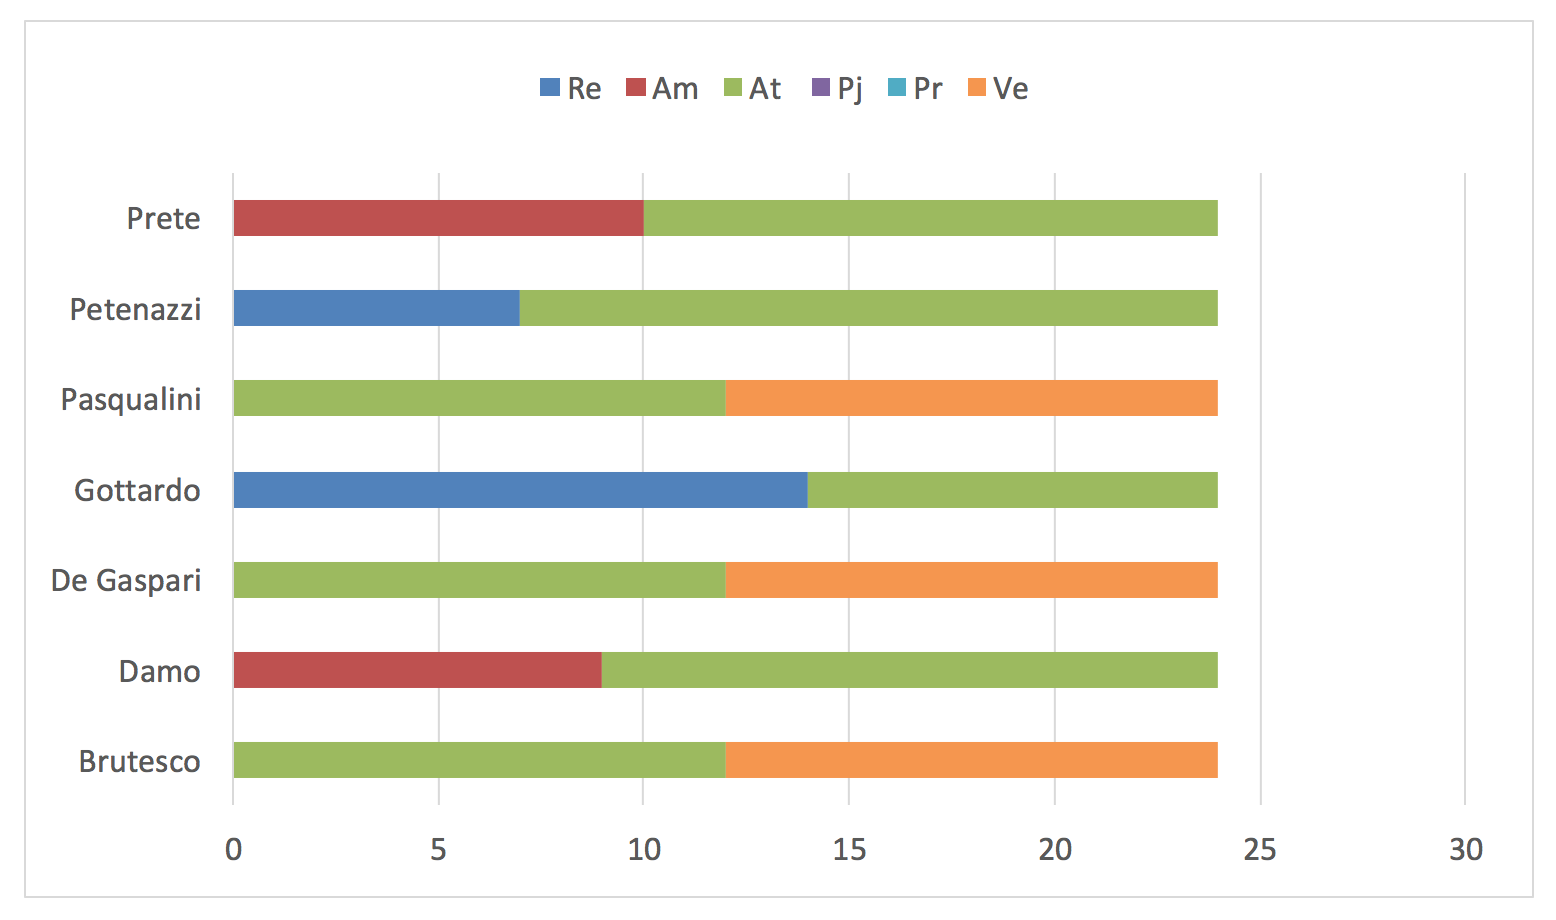
\includegraphics[scale=0.35]{img/h_An}
									\caption{Grafico del preventivo orario - Periodo: An}  \label{fig:h_An"} 		\end{figure}


%-----------------------------------------------------------------
			\begin{figure}[H]
			\centering
			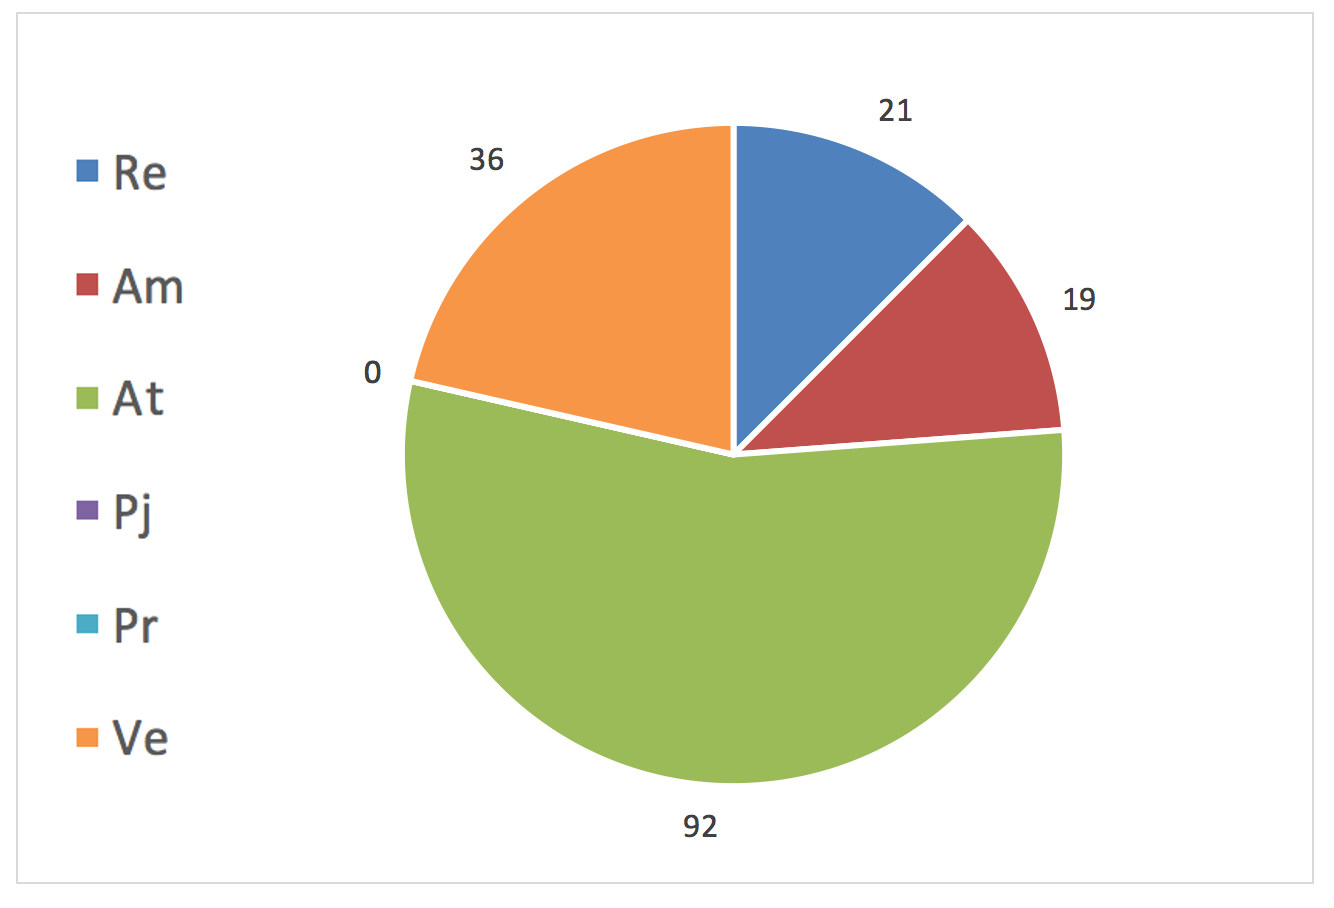
\includegraphics[scale=0.30]{img/h_r_An}
			\caption{Grafico del preventivo orario per ruolo - Periodo: An}
			\label{fig:h_r_An"}
			\end{figure}

		\newpage
			\paragraph{Preventivo economico}
		Le ore di questo periodo sono considerate solamente come ore di investimento e quindi non rendicontate.\\
%-----------------------------------------------------------------


							\begin{table}[H] \begin{center} \begin{tabular}{llllllll}
							\toprule
								&	\textbf{Re}	&	\textbf{Am}	&	\textbf{At}	&	\textbf{Pj}	&	\textbf{Pr}	&	\textbf{Ve}	&	\textbf{Tot}\\
							\midrule
							Tot in ore	&	21	&	19	&	92	&	0	&	0	&	36	&	168	 \\
							Tot. in €	&	 €     630,00 	 & 	 €  380,00 	 & 	 €  2.300,00 	 & 	 €           -   	 & 	 €               -   	 & 	 €  540,00 	 & 	 €        3.850,00 	 \\
							\bottomrule
							\end{tabular} \end{center} \caption{Prospetto economico - Periodo:
							An
							}\label{tab:s_An} \end{table}		\begin{figure}[H]  \centering  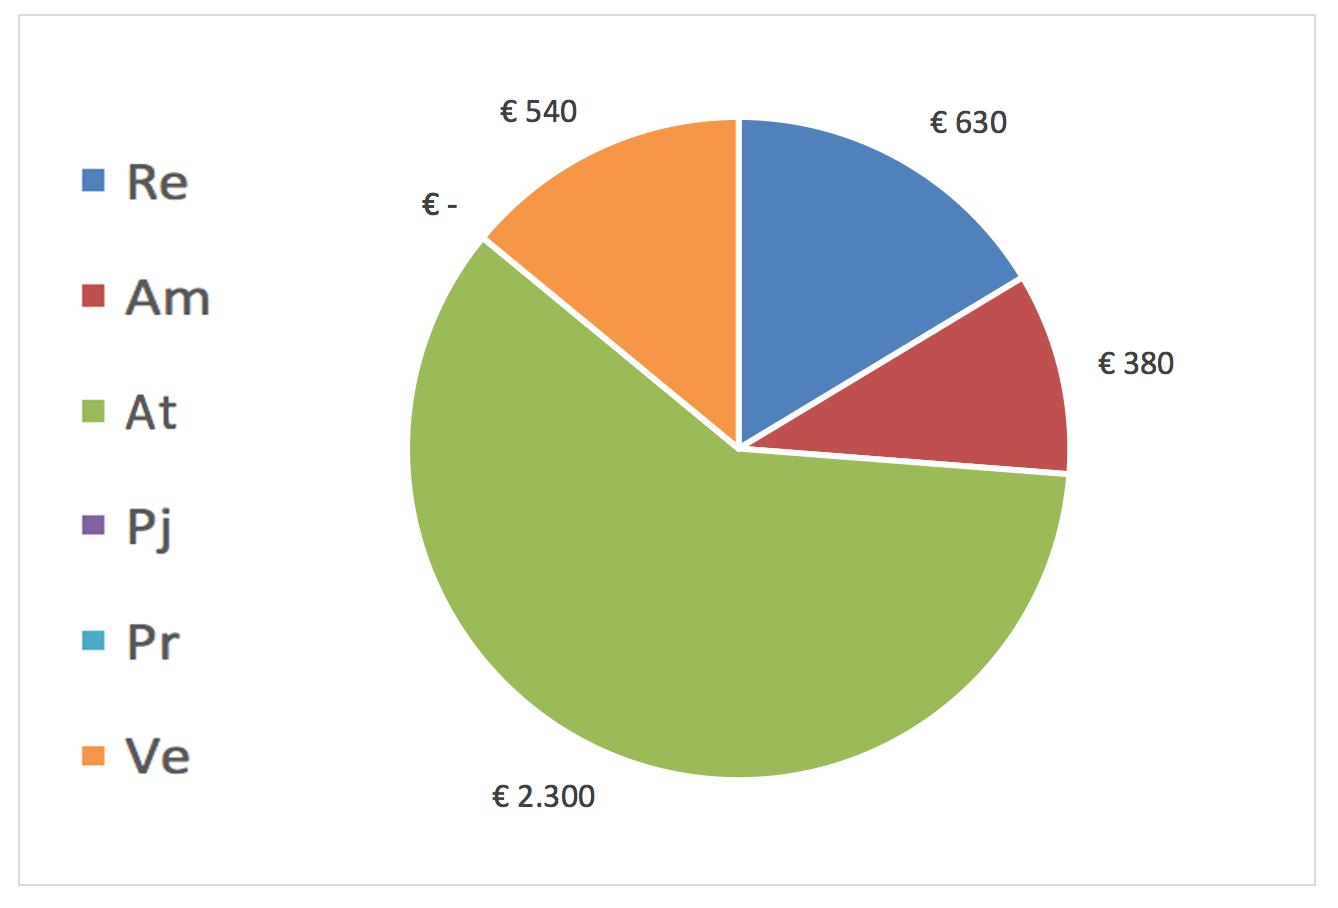
\includegraphics[scale=0.40]{img/s_An}
									\caption{Grafico del preventivo economico - Periodo: An}  \label{fig:s_An"} 		\end{figure}


%-----------------------------------------------------------------
		\newpage
		\subsubsection {Periodo: Pl - Progettazione logica}
		\paragraph{Preventivo orario}
%-----------------------------------------------------------------


							\begin{table}[H] \begin{center} \begin{tabular}{llllllll}
							\toprule
							\textbf{Nominativo}	&	\textbf{Re}	&	\textbf{Am}	&	\textbf{At}	&	\textbf{Pj}	&	\textbf{Pr}	&	\textbf{Ve}	&	\textbf{Tot}\\
							\midrule
							Brutesco	&	5	&	-	&	-	&	21	&	-	&	-	&	26	 \\
							Damo	&	5	&	-	&	-	&	30	&	-	&	-	&	35	 \\
							De Gaspari	&	-	&	-	&	-	&	10	&	-	&	16	&	26	 \\
							Gottardo	&	-	&	-	&	-	&	10	&	-	&	16	&	26	 \\
							Pasqualini	&	-	&	5	&	5	&	16	&	-	&	-	&	26	 \\
							Petenazzi	&	-	&	4	&	5	&	17	&	-	&	-	&	26	 \\
							Prete	&	-	&	-	&	-	&	10	&	-	&	16	&	26	 \\
							\midrule
							Tot in ore	&	10	&	9	&	10	&	114	&	0	&	48	&	191	 \\



							\bottomrule
							\end{tabular} \end{center} \caption{Prospetto orario - Periodo:
							Pl
							}\label{tab:h_Pl} \end{table}		\begin{figure}[H]  \centering  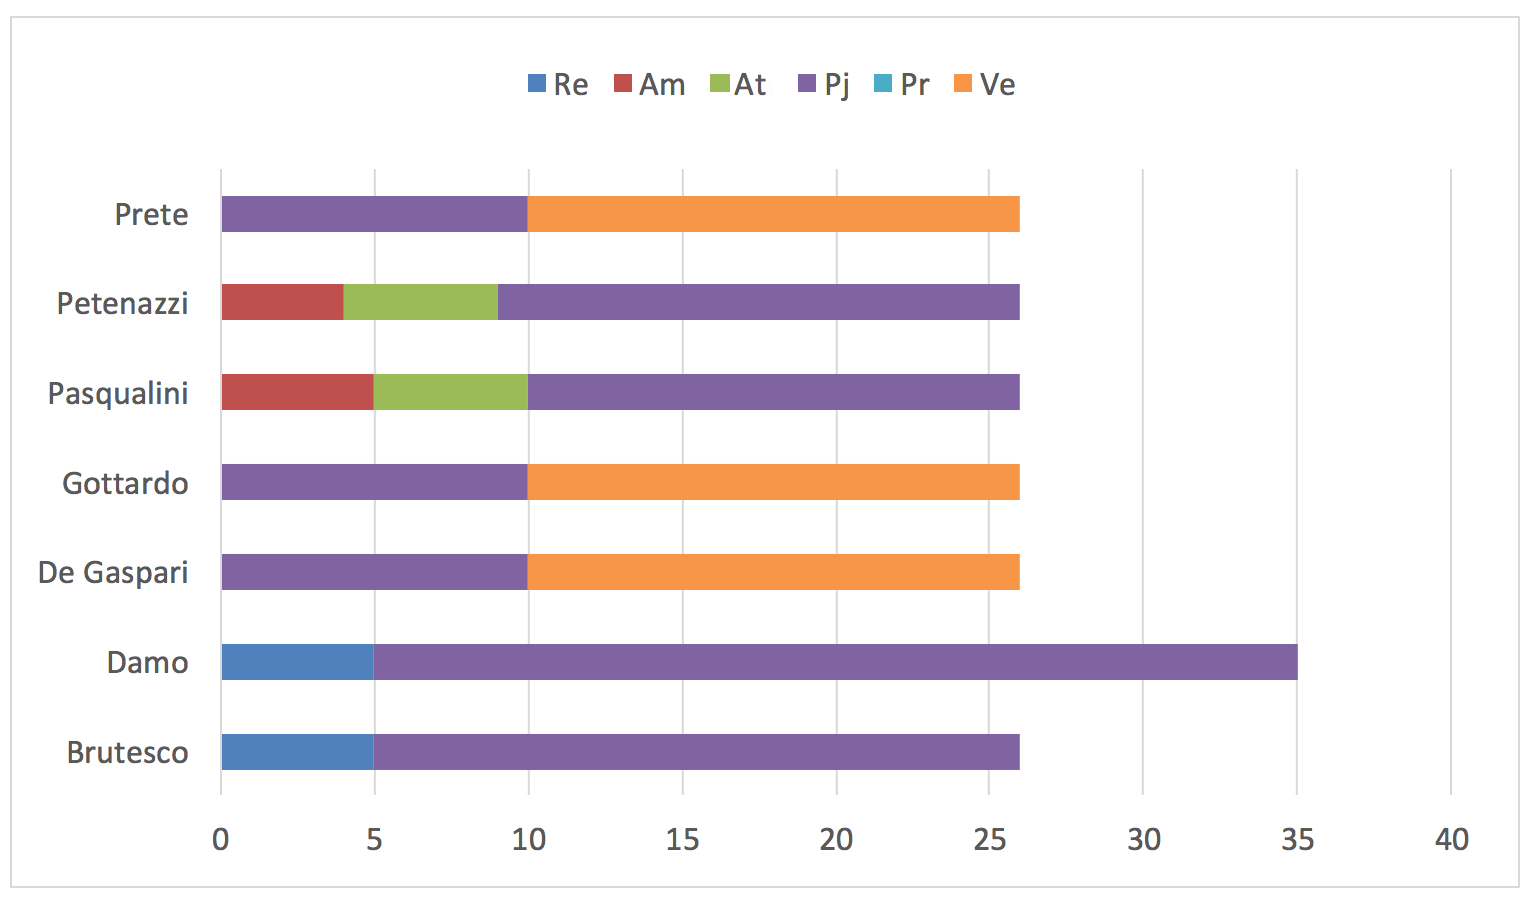
\includegraphics[scale=0.43]{img/h_Pl}
									\caption{Grafico del preventivo orario - Periodo: Pl}  \label{fig:h_Pl"} 		\end{figure}


%-----------------------------------------------------------------

			\begin{figure}[H]
			\centering
			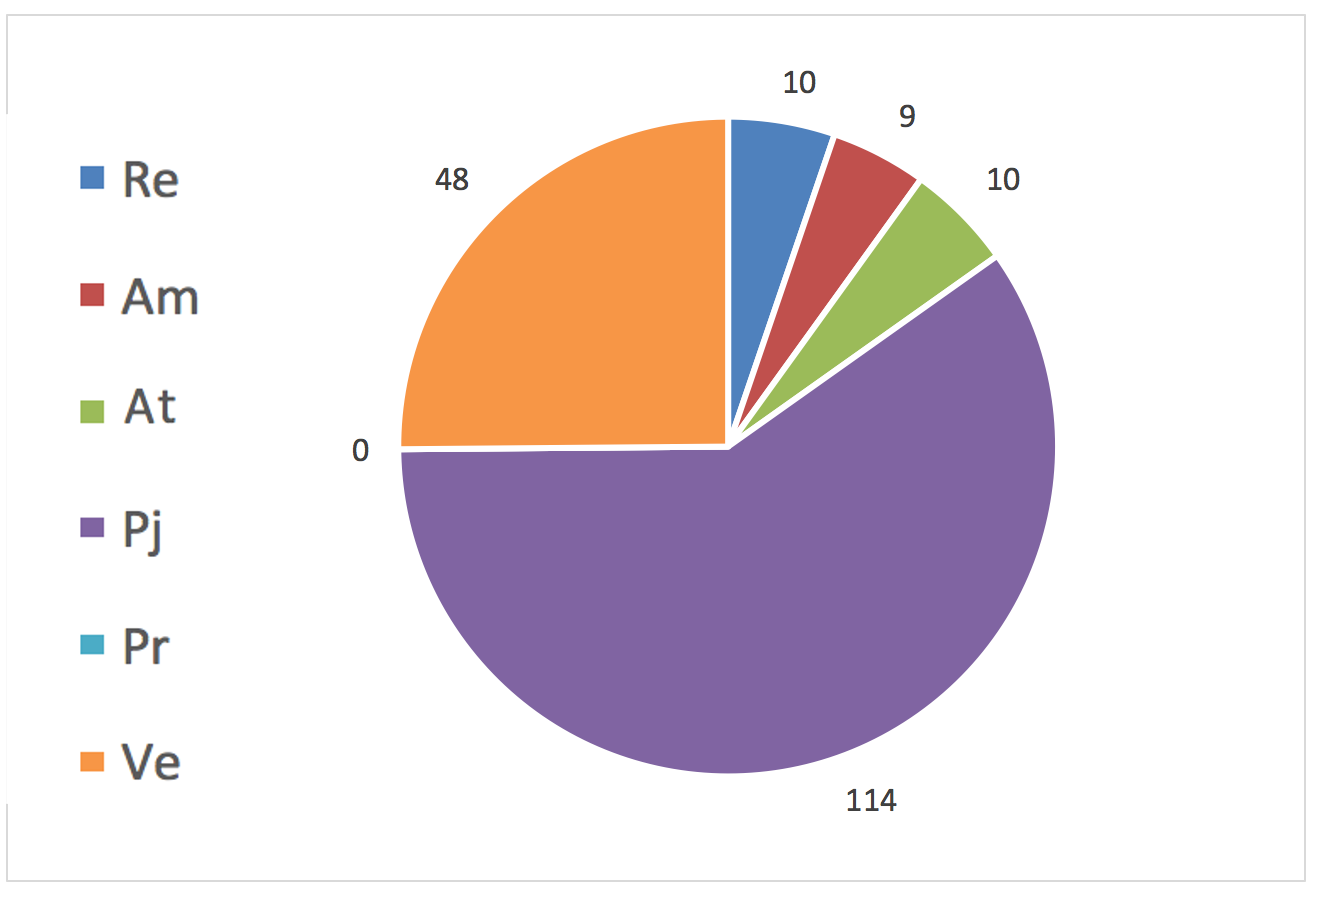
\includegraphics[scale=0.35]{img/h_r_Pl}
			\caption{Grafico del preventivo orario per ruolo - Periodo: Pl}
			\label{fig:h_r_Pl"}
			\end{figure}

			\newpage
			\paragraph{Preventivo economico}
			Il preventivo economico viene illustrato dalla tabella seguente. Le ore riportate sono tutte rendicontate.\\

%-----------------------------------------------------------------

							\begin{table}[H] \begin{center} \begin{tabular}{llllllll}
							\toprule
								&	\textbf{Re}	&	\textbf{Am}	&	\textbf{At}	&	\textbf{Pj}	&	\textbf{Pr}	&	\textbf{Ve}	&	\textbf{Tot}\\

							\midrule
							Tot in ore	&	10	&	9	&	10	&	114	&	0	&	48	&	191	 \\


							Tot in €	&	 €     300 	 & 	 €      180 	 & 	 €     250 	 & 	 €  2.508 	 & 	 €        -   	 & 	 €     720 	 & 	 €     3.958 	 \\
							\bottomrule
							\end{tabular} \end{center} \caption{Prospetto economico - Periodo:
							Pl
							}\label{tab:s_Pl} \end{table}


							\begin{figure}[H]  \centering  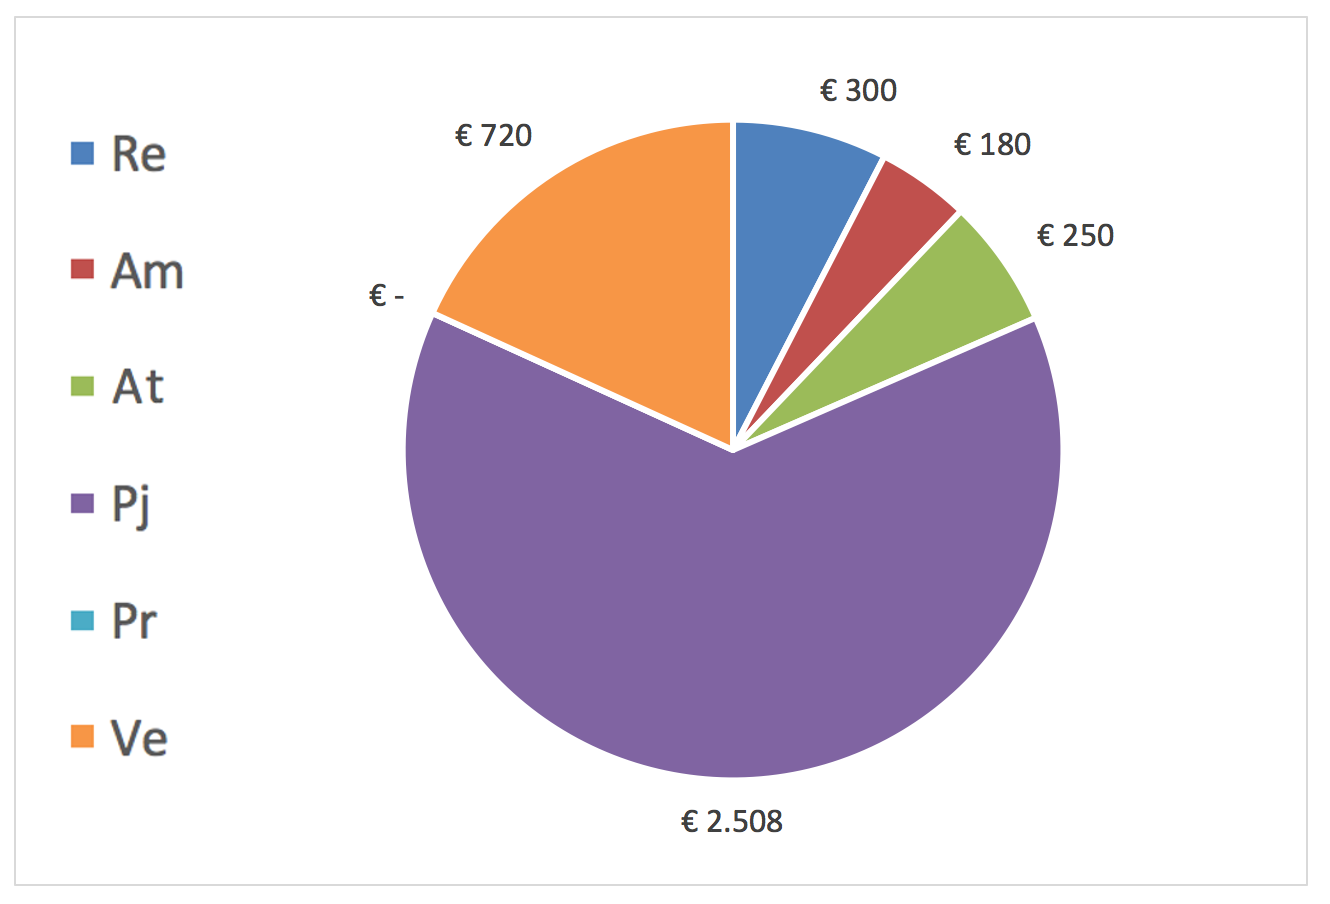
\includegraphics[scale=0.40]{img/s_Pl}
									\caption{Grafico del preventivo economico - Periodo: 								Pl	}  \label{fig:s_Pl"} 		\end{figure}
%-----------------------------------------------------------------
		\newpage
		\subsubsection {Periodo: PCV - Progettazione di dettaglio Codifica Validazione}
		\paragraph{Preventivo orario}
%-----------------------------------------------------------------

							\begin{table}[H] \begin{center} \begin{tabular}{llllllll}
							\toprule
							\textbf{Nominativo}	&	\textbf{Re}	&	\textbf{Am}	&	\textbf{At}	&	\textbf{Pj}	&	\textbf{Pr}	&	\textbf{Ve}	&	\textbf{Tot}\\
							\midrule
							Brutesco	&	-	&	4	&	-	&	5	&	15	&	29	&	53	 \\ 
							Damo	&	-	&		&	-	&	9	&	22	&	39	&	70	 \\ 
							De Gaspari	&	10	&	-	&	-	&	8	&	25	&	13	&	56	 \\ 
							Gottardo	&	-	&	6	&	-	&	28	&	22	&	-	&	56	 \\ 
							Pasqualini	&	-	&	4	&	-	&	29	&	16	&	7	&	56	 \\ 
							Petenazzi	&	-	&	5	&	-	&	12	&	20	&	19	&	56	 \\ 
							Prete	&	10	&	-	&	-	&	6	&	21	&	16	&	53	 \\ 
							\midrule															
							Tot in ore	&	20	&	19	&	0	&	97	&	141	&	123	&	400	 \\ 
							


							\bottomrule
							\end{tabular} \end{center} \caption{Prospetto orario - Periodo:
							PCV
							}\label{tab:h_PCV} \end{table}		\begin{figure}[H]  \centering  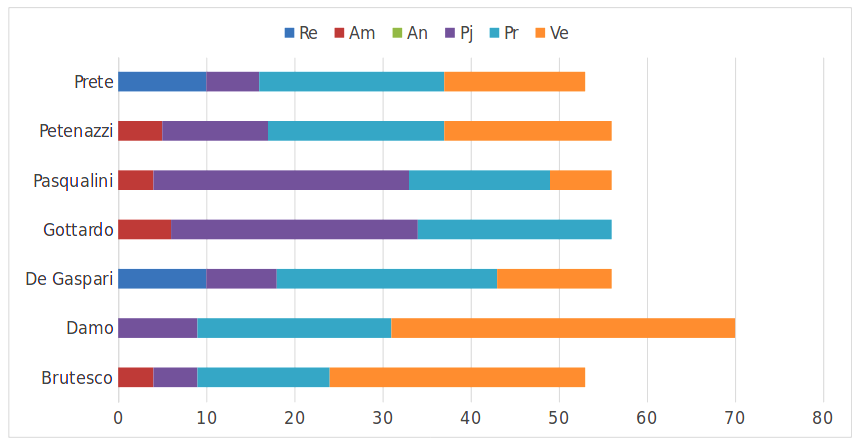
\includegraphics[scale=0.37]{img/h_PCV}
									\caption{Grafico del preventivo orario - Periodo: 								PCV	}  \label{fig:h_PCV} \end{figure}

%-----------------------------------------------------------------
			\begin{figure}[H]
			\centering
			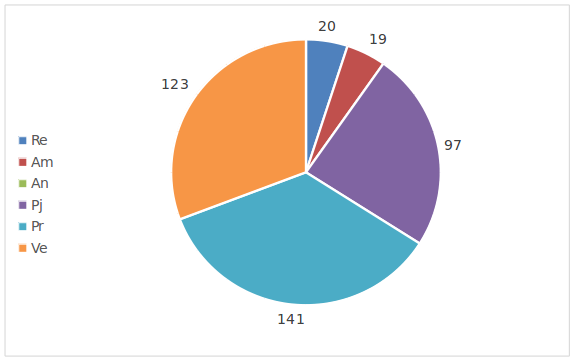
\includegraphics[scale=0.42]{img/h_r_PCV}
			\caption{Grafico del preventivo orario per ruolo - Periodo: PCV}
			\label{fig:h_r_PCV"}
			\end{figure}

			\newpage
			\paragraph{Preventivo economico}
			Il preventivo economico viene illustrato dalla tabella seguente. Le ore riportate sono tutte rendicontate.\\
%-----------------------------------------------------------------

							\begin{table}[H] \begin{center} \begin{tabular}{llllllll}
							\toprule
								&	\textbf{Re}	&	\textbf{Am}	&	\textbf{At}	&	\textbf{Pj}	&	\textbf{Pr}	&	\textbf{Ve}	&	\textbf{Tot}\\

							\midrule
							Tot in ore	&	20	&	19	&	0	&	97	&	141	&	123	&	400	 \\ 
							Tot in €	&	 € 600 	 & 	 € 380 	 & 	 € -   	 & 	 € 2.134 	 & 	 € 2.115 	 & 	 € 1.845 	 & 	 € 7.074 	 \\ 
							\bottomrule
							\end{tabular} \end{center} \caption{Prospetto economico - Periodo:
							PCV
							}\label{tab:s_PCV} \end{table}		\begin{figure}[H]  \centering  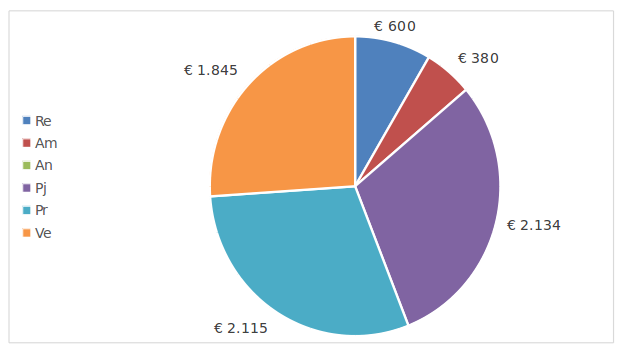
\includegraphics[scale=0.40]{img/s_PCV.png}
									\caption{Grafico del preventivo economico - Periodo: 								PCV	}  \label{fig:s_PCV} \end{figure}

%-----------------------------------------------------------------
		\newpage
		\subsubsection {Periodo: Va - Validazione}
		\paragraph{Preventivo orario}
%-----------------------------------------------------------------

							\begin{table}[H] \begin{center} \begin{tabular}{llllllll}
							\toprule
							\textbf{Nominativo}		&	\textbf{Re}	&	\textbf{Am}	&	\textbf{At}	&	\textbf{Pj}	&	\textbf{Pr}	&	\textbf{Ve}	&	\textbf{Tot}\\
							\midrule
							Brutesco	&	-	&	-	&	-	&	-	&	6	&	20	&	26	 \\
							Damo	&	-	&	-	&	-	&	-	&	-	&	-	&	0	 \\
							De Gaspari	&	-	&	10	&	-	&	-	&	-	&	13	&	23	 \\
							Gottardo	&	-	&	-	&	-	&	-	&	6	&	17	&	23	 \\
							Pasqualini	&	13	&	-	&	-	&	-	&	-	&	10	&	23	 \\
							Petenazzi	&	-	&	-	&	-	&	-	&	7	&	16	&	23	 \\
							Prete	&	-	&	-	&	-	&	-	&	11	&	15	&	26	 \\
							\midrule
							Tot in ore	&	13	&	10	&	0	&	0	&	30	&	91	&	144	 \\


							\bottomrule
							\end{tabular} \end{center} \caption{Prospetto orario - Periodo:
							Va
							}\label{tab:h_Va} \end{table}		\begin{figure}[H]  \centering  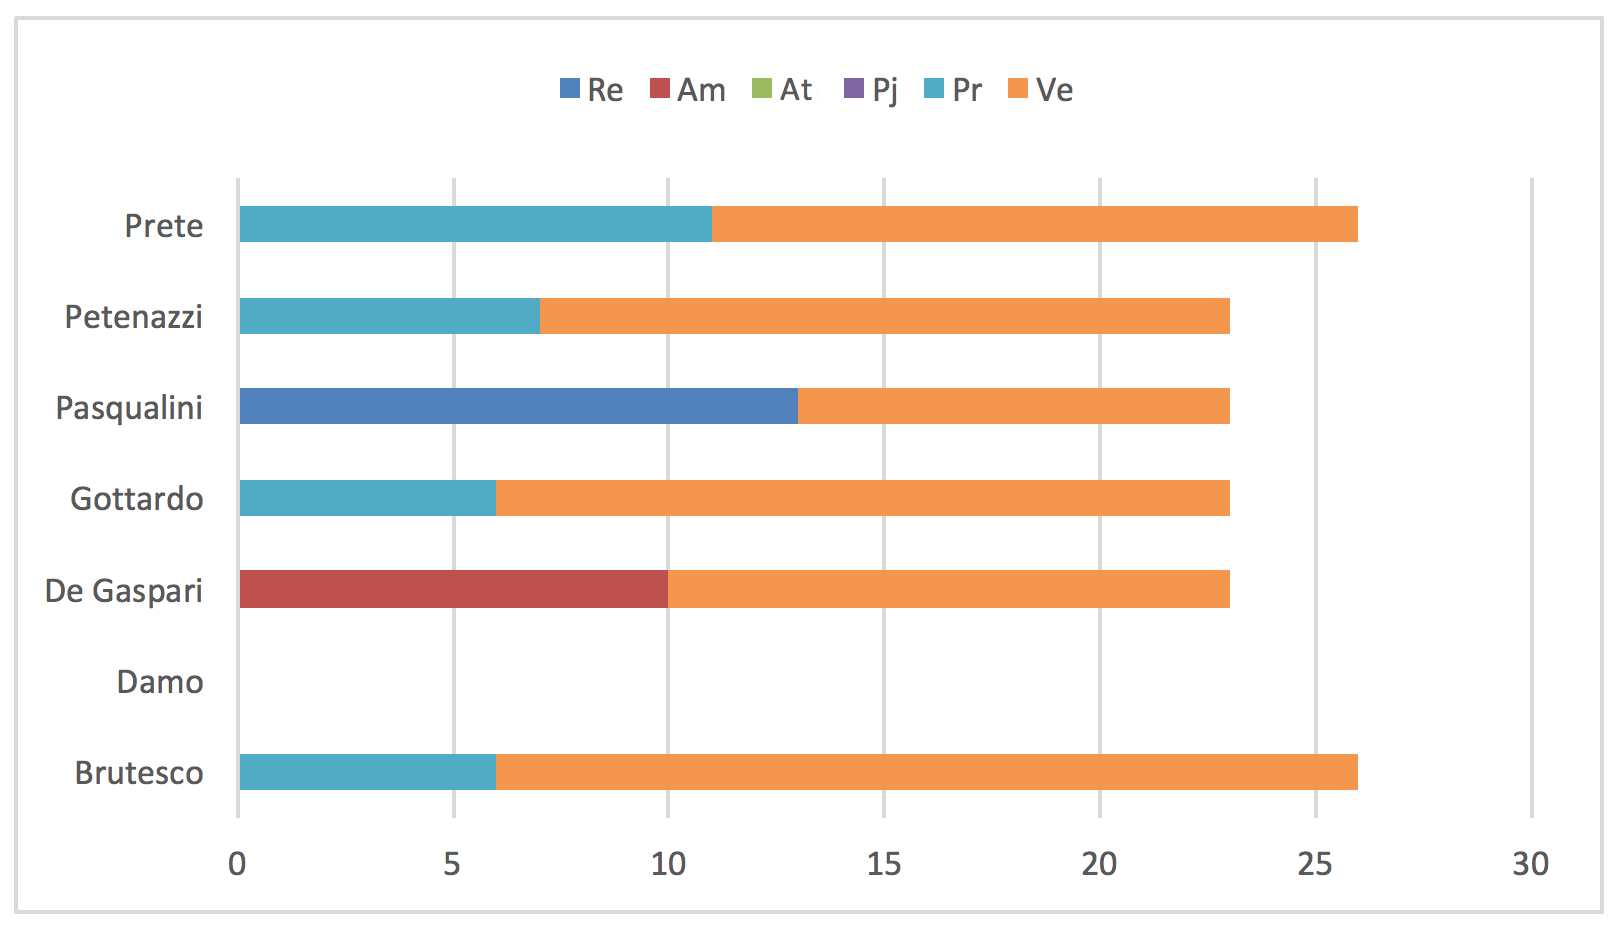
\includegraphics[scale=0.42]{img/h_Va}
									\caption{Grafico del preventivo orario - Periodo: 								Va	}  \label{fig:h_Va	} \end{figure}
%-----------------------------------------------------------------
			\begin{figure}[H]
			\centering
			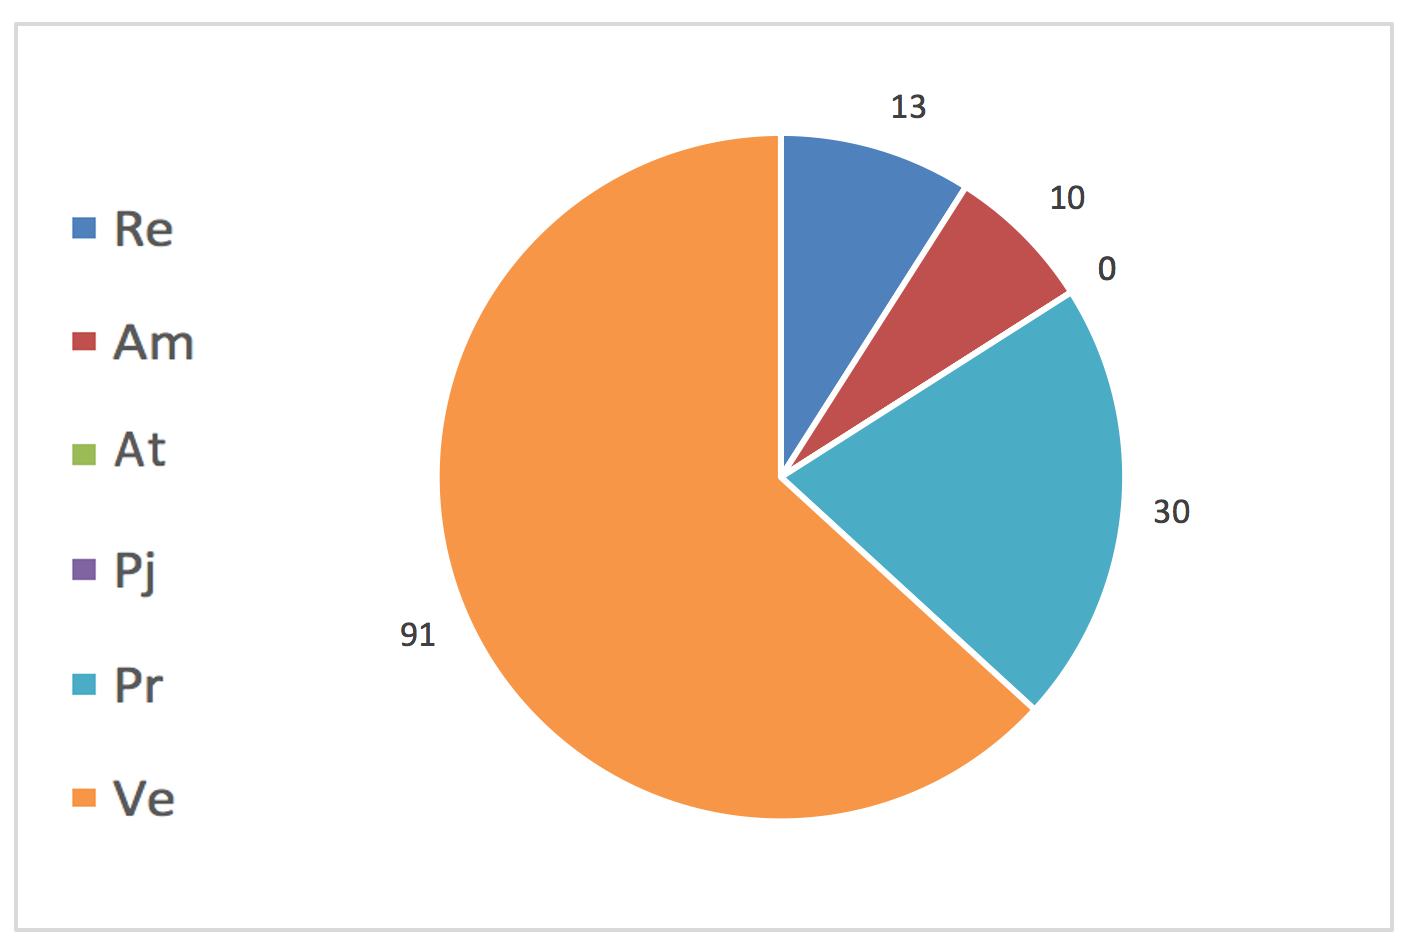
\includegraphics[scale=0.32]{img/h_r_Va}
			\caption{Grafico del preventivo orario per ruolo - Periodo: Va}
			\label{fig:Va"}
			\end{figure}

			\newpage
			\paragraph{Preventivo economico}
			Il preventivo economico viene illustrato dalla tabella seguente. Le ore riportate sono tutte rendicontate.\\

%-----------------------------------------------------------------

							\begin{table}[H] \begin{center} \begin{tabular}{llllllll}
							\toprule
								&	\textbf{Re}	&	\textbf{Am}	&	\textbf{At}	&	\textbf{Pj}	&	\textbf{Pr}	&	\textbf{Ve}	&	\textbf{Tot}\\

							\midrule
							Tot in ore	&	13	&	10	&	0	&	0	&	30	&	91	&	144	 \\


							Tot in €	&	 €     390 	 & 	 €      200 	 & 	 €         -   	 & 	 €         -   	 & 	 €    450 	 & 	 €  1.365 	 & 	 €     2.405 	 \\
							\bottomrule
							\end{tabular} \end{center} \caption{Prospetto economico - Periodo:
							Va
							}\label{tab:s_Va} \end{table}		\begin{figure}[H]  \centering  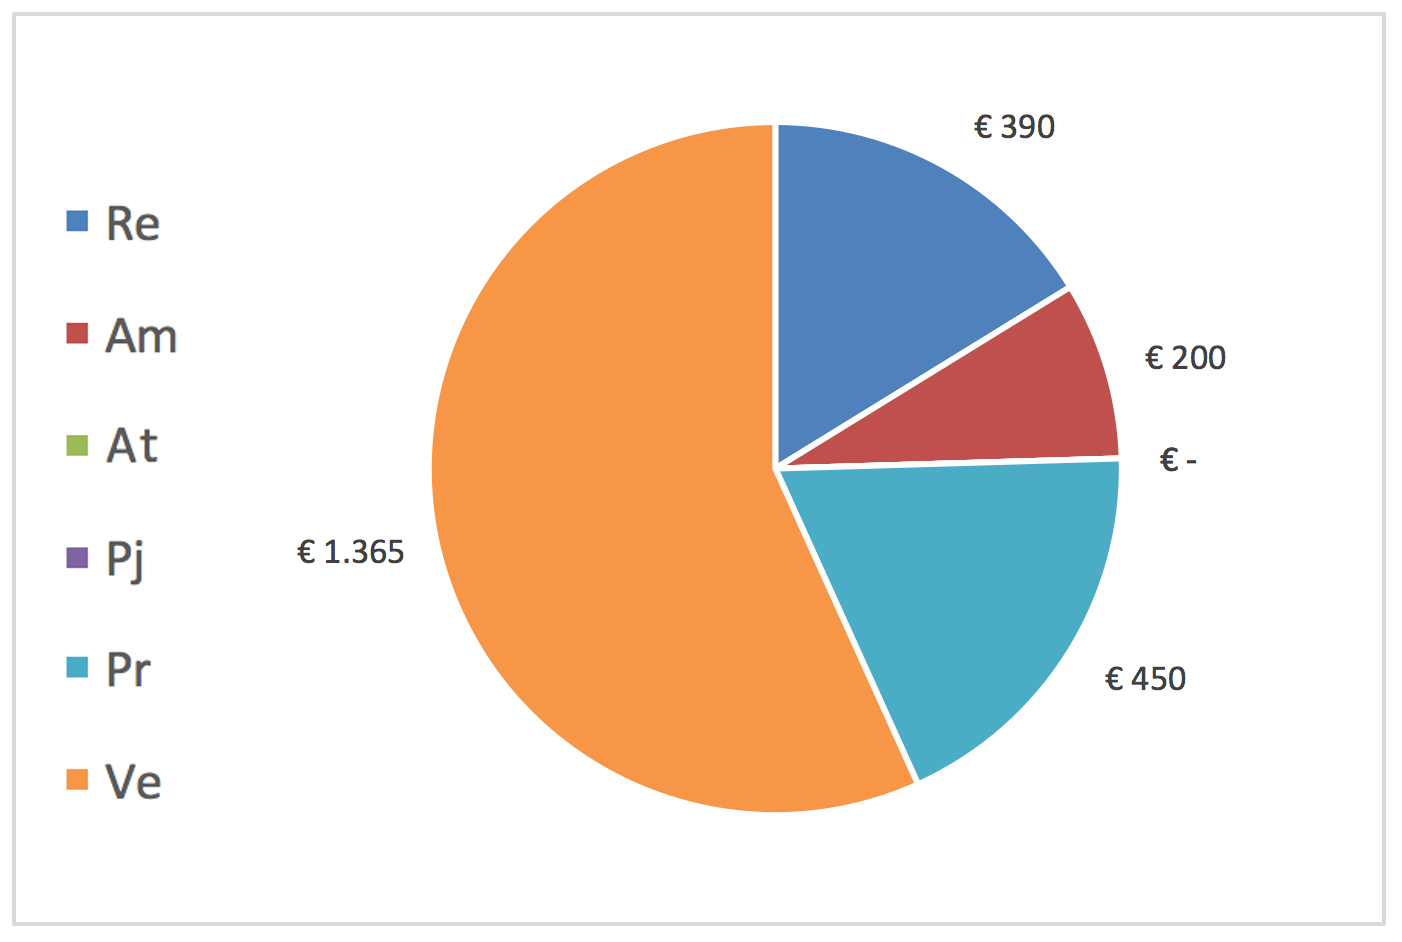
\includegraphics[scale=0.40]{img/s_Va}
									\caption{Grafico del preventivo economico - Periodo: 								Va	}  \label{fig:s_Va	} \end{figure}

%-----------------------------------------------------------------
	\newpage
	\subsection {Totale non rendicontato}
		\subsubsection {Preventivo orario}
		Si stima inoltre che ogni membro del \glo{Gruppo}{gruppo} dedicherà per ogni ruolo un numero di ore non rendicontate di investimento pari a:\\
		\begin{table}[H] \begin{center} \begin{tabular}{lllllll}
		\toprule
			Re	&	Am	&	An	&	Pj	&	Pr	&	Ve	&	Tot	 \\
		\midrule
			2	&	3	&	2	&	2	&	2	&	2	&	13	 \\
		\bottomrule
		\end{tabular} \end{center}
		\caption{Ulteriori ore non rendicontate}
		\label{tab:h_ulteriori}
        \end{table}\mbox{}\\

		Quindi, durante l'intero arco dello sviluppo del progetto, le ore non rendicontate ammontano a:\\
%-----------------------------------------------------------------

							\begin{table}[H] \begin{center} \begin{tabular}{llllllll}
							\toprule
							\textbf{Nominativo}	&	\textbf{Re}	&	\textbf{Am}	&	\textbf{At}	&	\textbf{Pj}	&	\textbf{Pr}	&	\textbf{Ve}	&	\textbf{Tot}\\
							\midrule
							Brutesco	&	2	&	3	&	14	&	2	&	2	&	14	&	37	 \\
							Damo		&	2	&	12	&	17	&	2	&	2	&	2	&	37	 \\
							De Gaspari	&	2	&	3	&	14	&	2	&	2	&	14	&	37	 \\
							Gottardo	&	16	&	3	&	12	&	2	&	2	&	2	&	37	 \\
							Pasqualini	&	2	&	3	&	14	&	2	&	2	&	14	&	37	 \\
							Petenazzi	&	9	&	3	&	19	&	2	&	2	&	2	&	37	 \\
							Prete		&	2	&	13	&	16	&	2	&	2	&	2	&	37	 \\
							\midrule
							Tot in ore	&	35	&	40	&	106	&	14	&	14	&	50	&	259	 \\
							\bottomrule
							\end{tabular} \end{center}
							\caption{Prospetto riassuntivo delle ore non rendicontate}
							\label{tab:h_TotaleNonRendicontato} \end{table}\mbox{}\\

							\begin{figure}[H]  \centering
							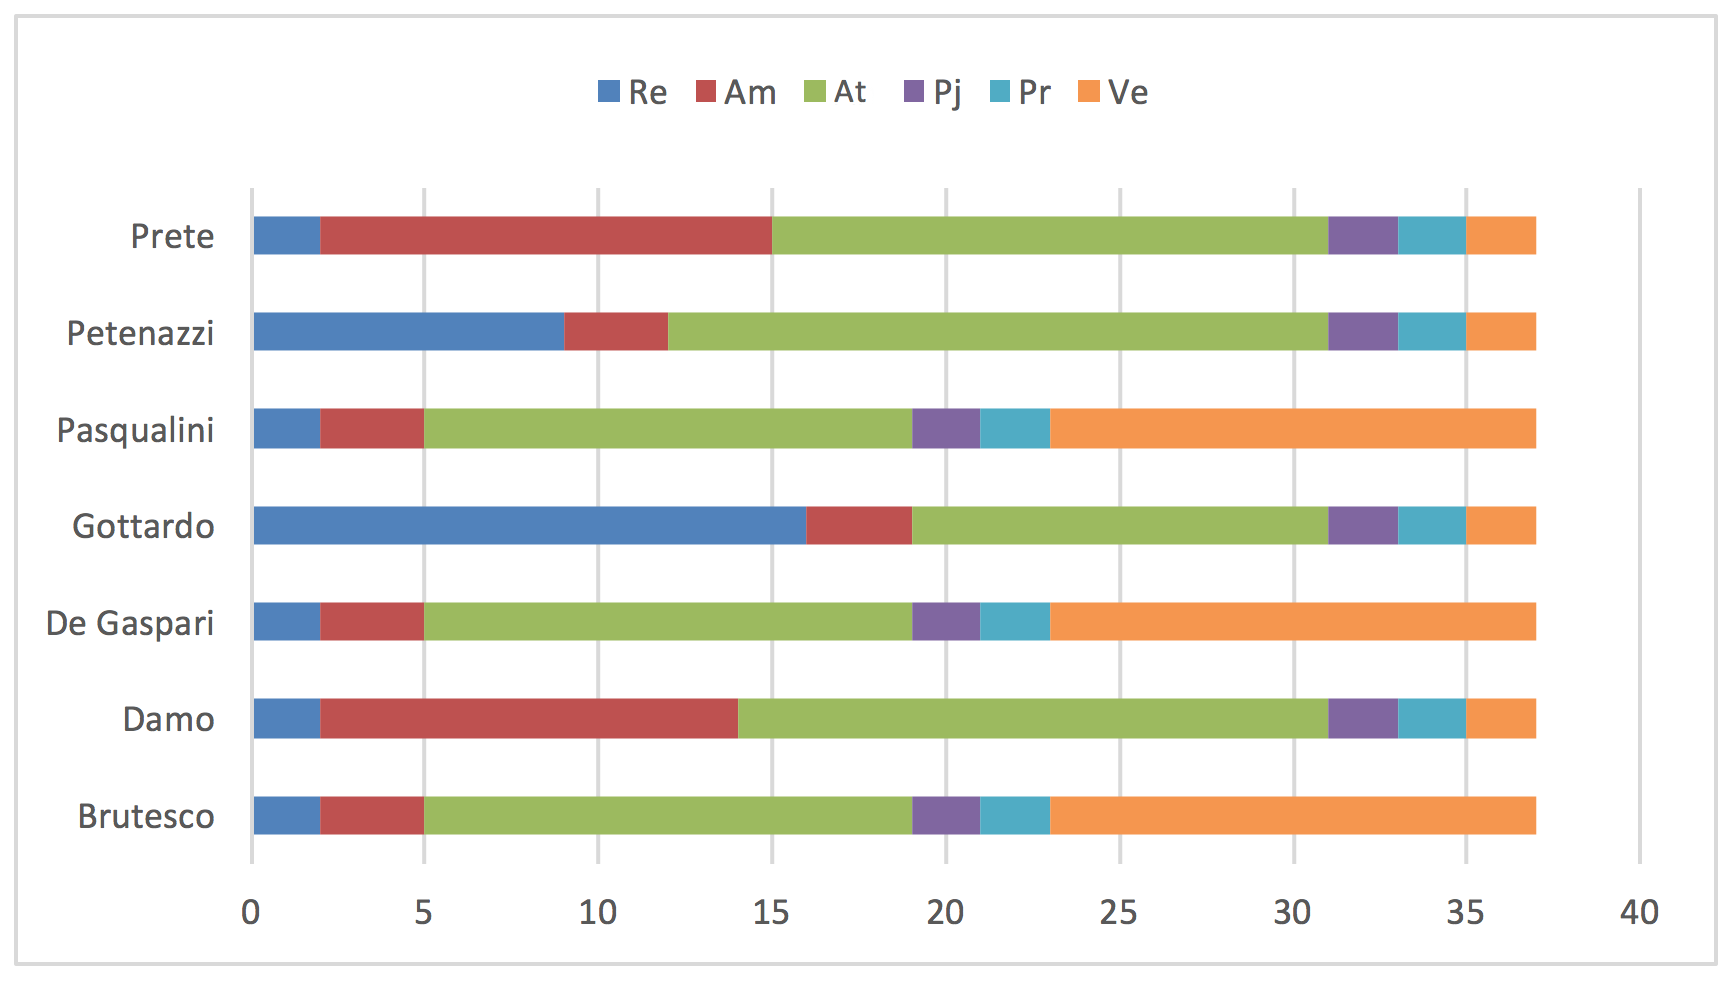
\includegraphics[width=\textwidth]{img/h_NonRend}
							\caption{Grafico riassuntivo delle ore non rendicontate}
							\label{fig:h_non_rend"} 		\end{figure}
%-----------------------------------------------------------------
			\begin{figure}[H]
			\centering
			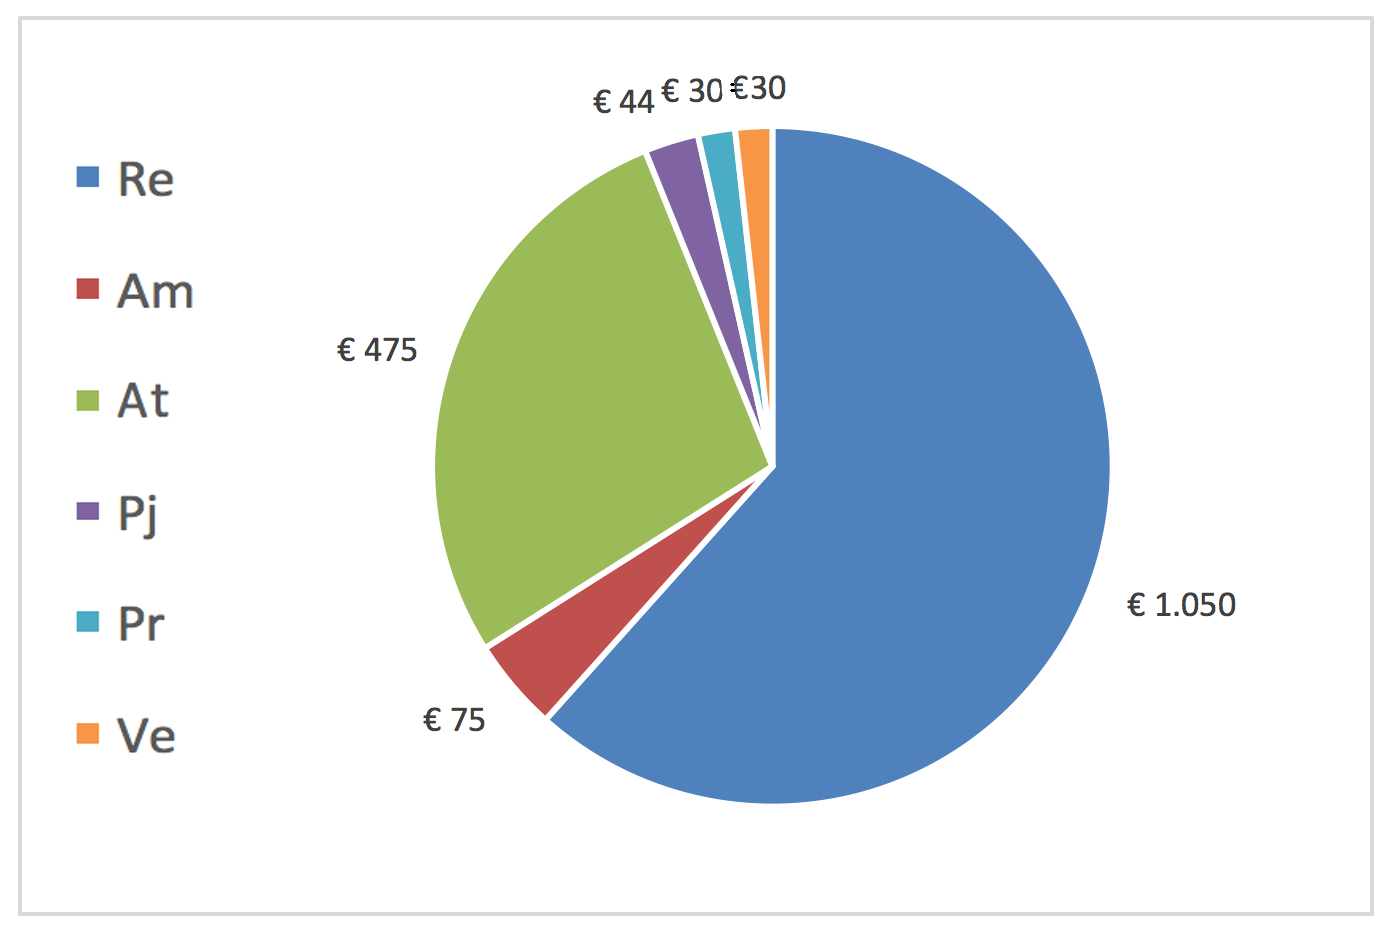
\includegraphics[scale=0.40]{img/h_r_TotaleNonRendicontato}
			\caption{Grafico del preventivo orario per ruolo - Totale non rendicontato}
			\label{fig:Totale non rendicontato"}
			\end{figure}
%-----------------------------------------------------------------
			\begin{figure}[H]
			\centering
			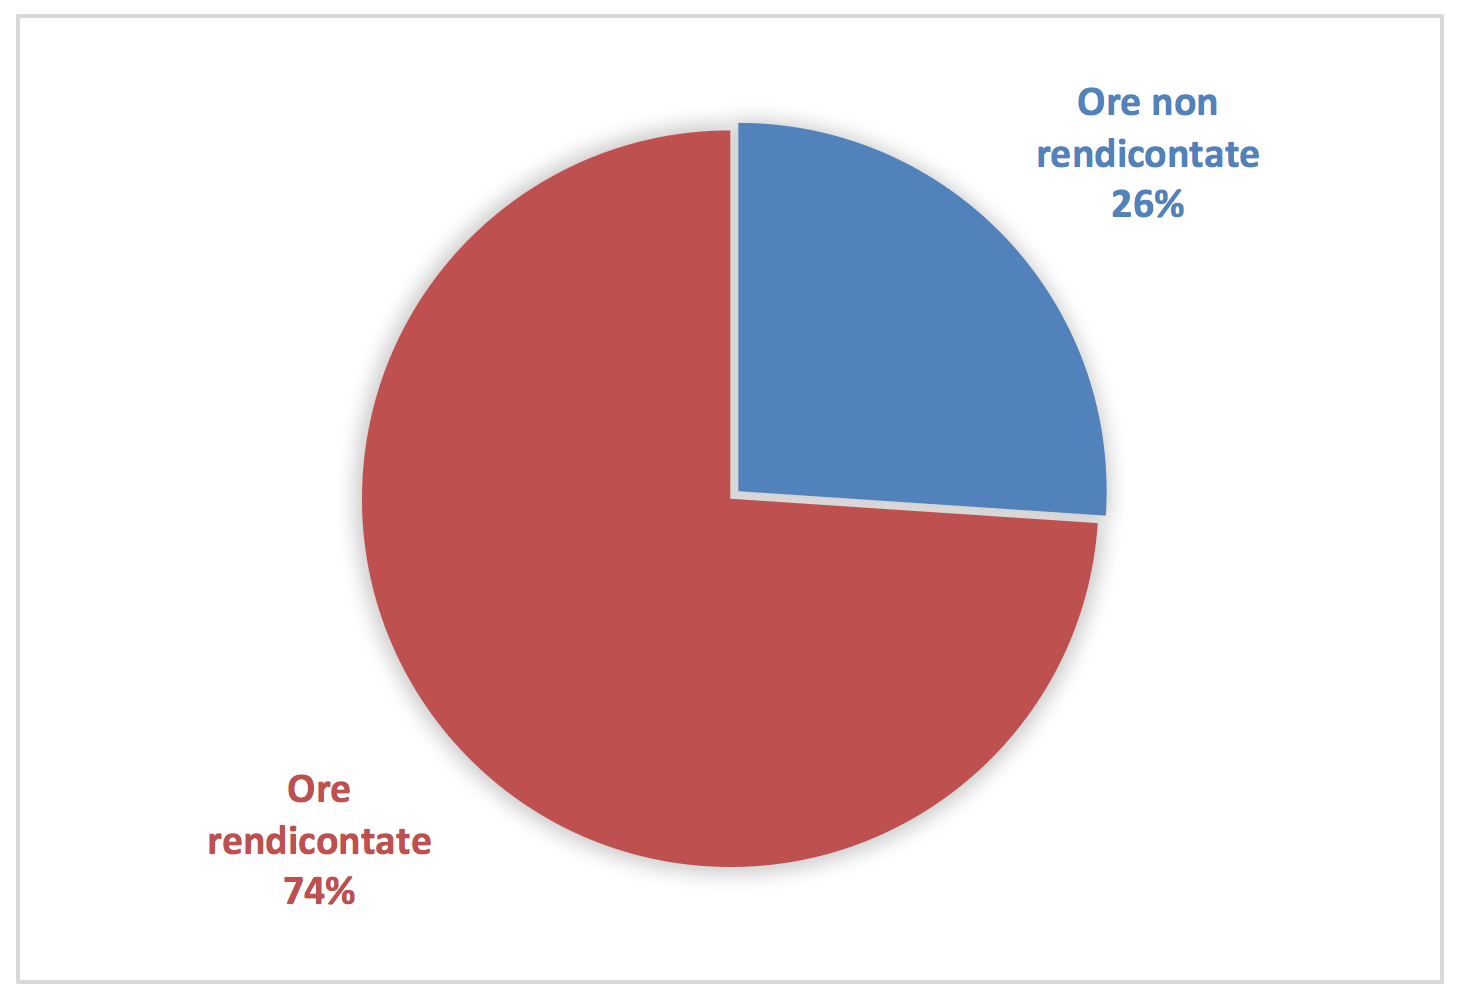
\includegraphics[scale=0.40]{img/incidenza}
			\caption{Incidenza delle ore non rendicontate sul totale delle ore complessivo}
			\label{fig:incidenza}
			\end{figure}
%-----------------------------------------------------------------
			\newpage
			\subsubsection {Preventivo economico}
%-----------------------------------------------------------------
			\begin{table}[H] \begin{center} \begin{tabular}{llllllll}
			\toprule
				&	\textbf{Re}	&	\textbf{Am}	&	\textbf{At}	&	\textbf{Pj}	&	\textbf{Pr}	&	\textbf{Ve}	&	\textbf{Tot}\\

			\midrule
			Tot in ore	&	35	&	40	&	106	&	14	&	14	&	50	&	259	 \\


			Tot in €	&	 €        1.050 	 & 	 €        800 	 & 	 €        2.650 	 & 	 €        308 	 & 	 €            210 	 & 	 €        750 	 & 	 €              5.768 	 \\
			\bottomrule
			\end{tabular} \end{center} \caption{Prospetto economico -
			Totale non rendicontato
			}\label{tab:s_TotaleNonRendicontato} \end{table}
%-----------------------------------------------------------------
			\begin{figure}[H]
			\centering
			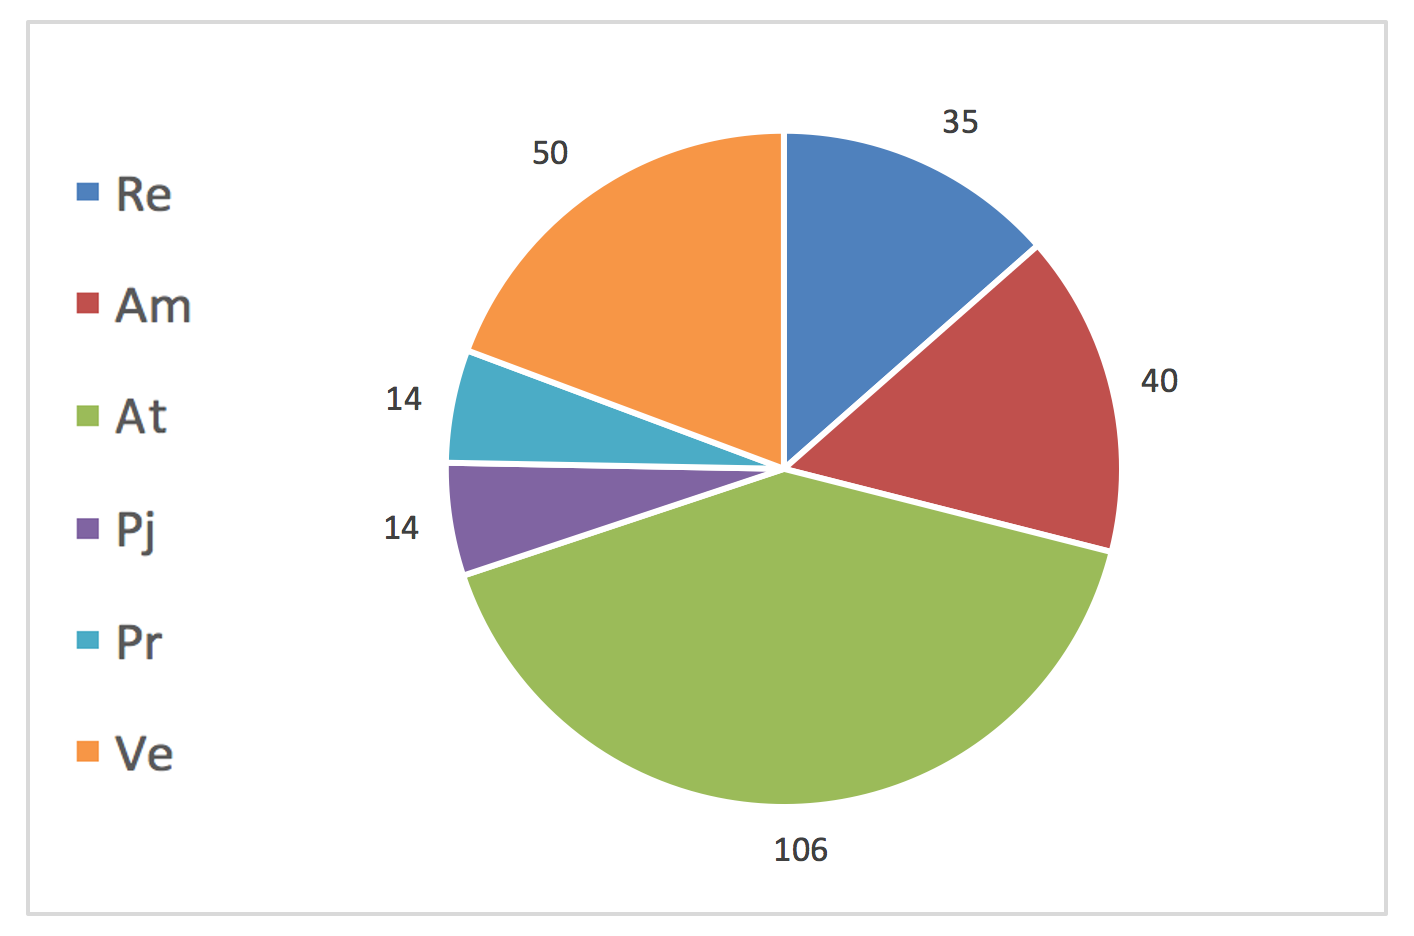
\includegraphics[scale=0.40]{img/s_TotaleNonRendicontato}
			\caption{Grafico del preventivo economico per ruolo - Totale non rendicontato}
			\label{fig:TotaleNonRendicontato}
			\end{figure}
%-----------------------------------------------------------------
		\newpage
		\subsection {Totale complessivo}
				\subsubsection {Preventivo orario}
		Durante l'intero arco dello sviluppo del progetto, includendo anche le ore non rendicontate, i membri del gruppo ricopriranno i vari ruoli secondo la seguente suddivisione:\\
%-----------------------------------------------------------------

								\begin{table}[H] \begin{center} \begin{tabular}{llllllll}
								\toprule
								\textbf{Nominativo}	&	\textbf{Re}	&	\textbf{Am}	&	\textbf{At}	&	\textbf{Pj}	&	\textbf{Pr}	&	\textbf{Ve}	&	\textbf{Tot}\\
								\midrule
								Brutesco	&	7	&	7	&	14	&	28	&	23	&	63	&	142	 \\
								Damo	&	7	&	12	&	17	&	41	&	24	&	41	&	142	 \\
								De Gaspari	&	12	&	13	&	14	&	20	&	27	&	56	&	142	 \\
								Gottardo	&	16	&	9	&	12	&	40	&	30	&	35	&	142	 \\
								Pasqualini	&	15	&	12	&	19	&	47	&	18	&	31	&	142	 \\
								Petenazzi	&	9	&	12	&	24	&	31	&	29	&	37	&	142	 \\
								Prete	&	12	&	13	&	16	&	18	&	34	&	49	&	142	 \\
								\midrule
								Tot in ore	&	78	&	78	&	116	&	225	&	185	&	312	&	994	 \\



								\bottomrule
								\end{tabular} \end{center} \caption{Prospetto orario -
								Totale complessivo
								}\label{tab:h_TotaleComplessivo} \end{table}\mbox{}\\
                        		\begin{figure}[H]  \centering  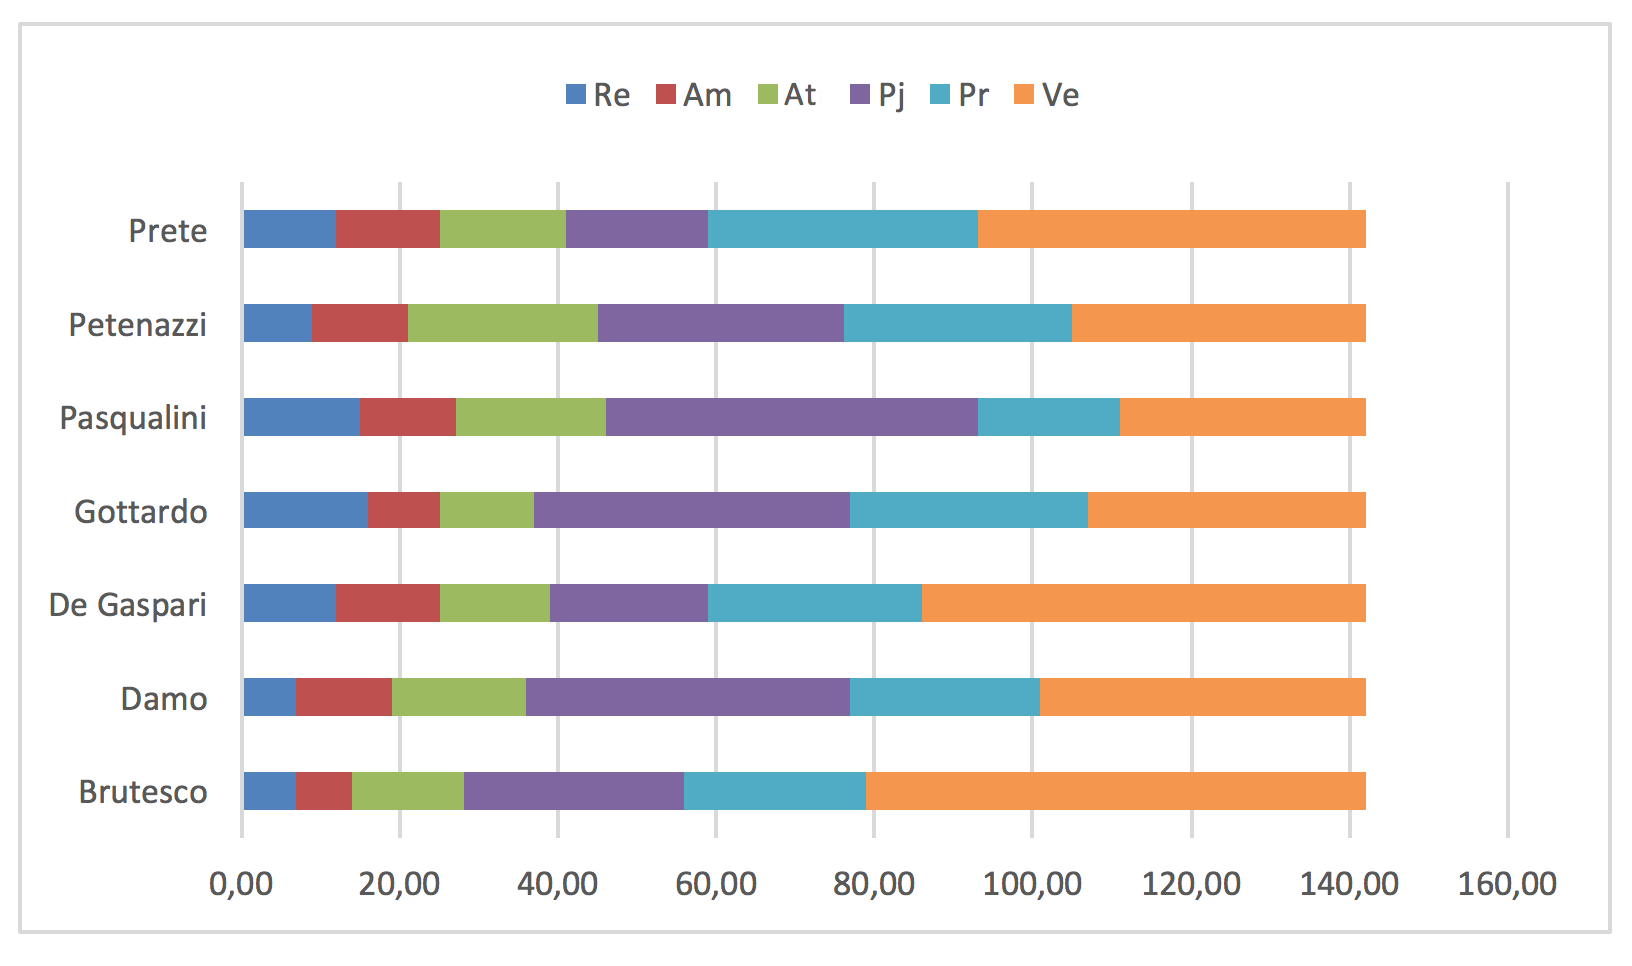
\includegraphics[scale=0.40]{img/h_Totale}
										\caption{Grafico del preventivo orario - 								Totale complessivo	}  \label{fig:h_TotaleComplessivo} \end{figure}
%-----------------------------------------------------------------
			\begin{figure}[H]
			\centering
			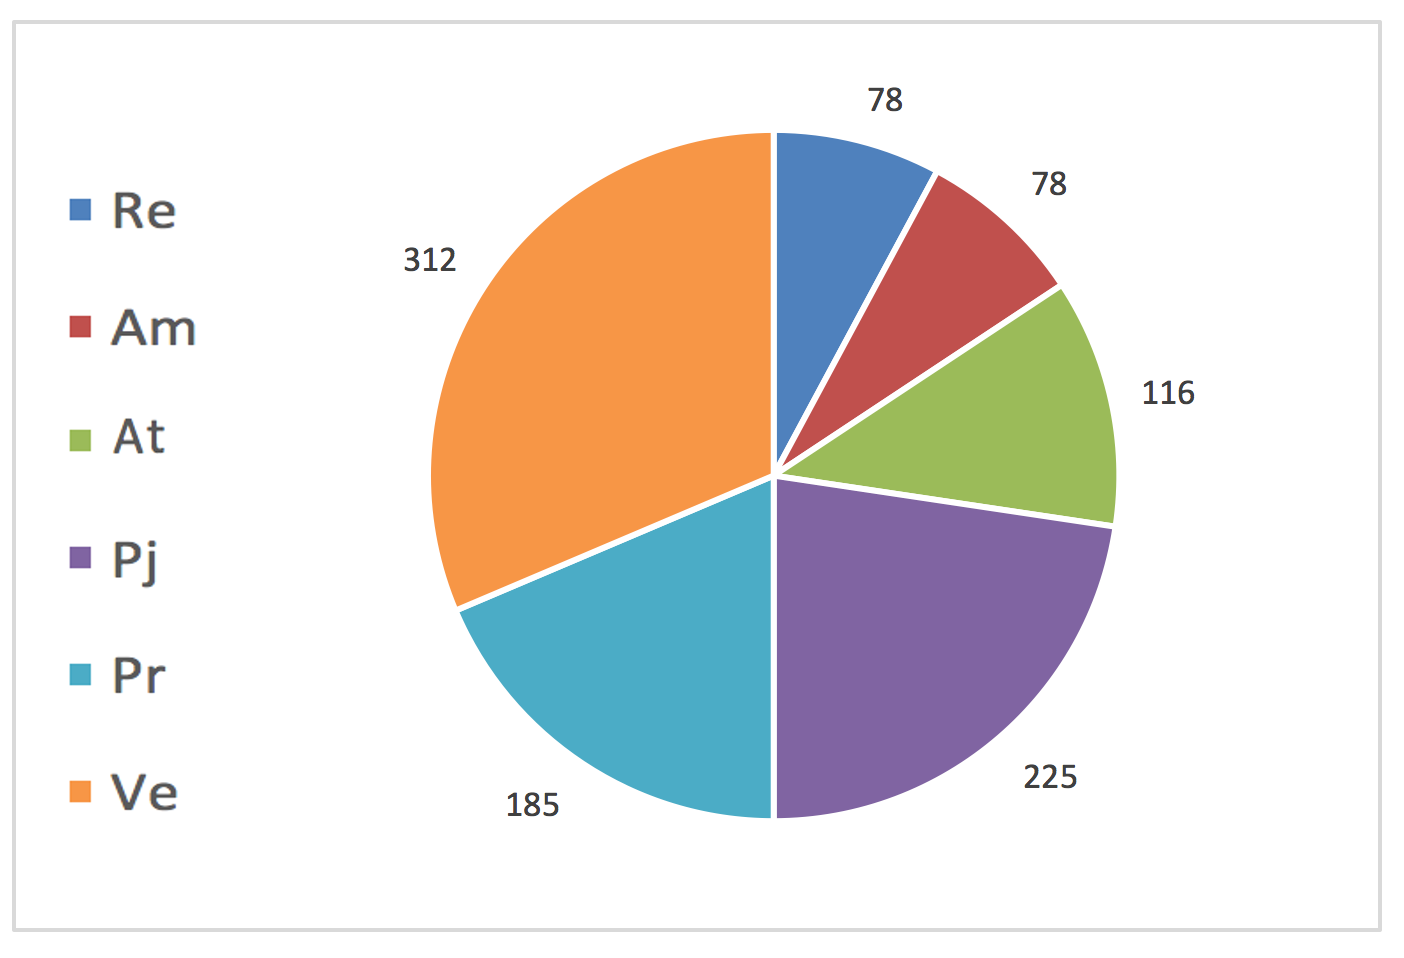
\includegraphics[scale=0.40]{img/h_r_Totale}
			\caption{Grafico del preventivo orario per ruolo - Totale complessivo}
			\label{fig:Totale complessivo orario}
			\end{figure}
					\newpage
					\subsubsection {Preventivo economico}
%-----------------------------------------------------------------

								\begin{table}[H] \begin{center} \begin{tabular}{llllllll}
								\toprule
									&	\textbf{Re}	&	\textbf{Am}	&	\textbf{At}	&	\textbf{Pj}	&	\textbf{Pr}	&	\textbf{Ve}	&	\textbf{Tot}\\
								\midrule
								Tot in ore	&	78	&	78	&	116	&	225	&	185	&	312	&	994	 \\


								Tot in €	&	 €        2.340 	 & 	 €    1.560 	 & 	 €        2.900 	 & 	 €    4.950 	 & 	 €        2.775 	 & 	 €    4.680 	 & 	 €           19.205 	 \\
								\bottomrule
								\end{tabular} \end{center} \caption{Prospetto economico -
								Totale complessivo
								}\label{tab:s_TotaleComplessivo} \end{table}

%-----------------------------------------------------------------
			\begin{figure}[H]
			\centering
			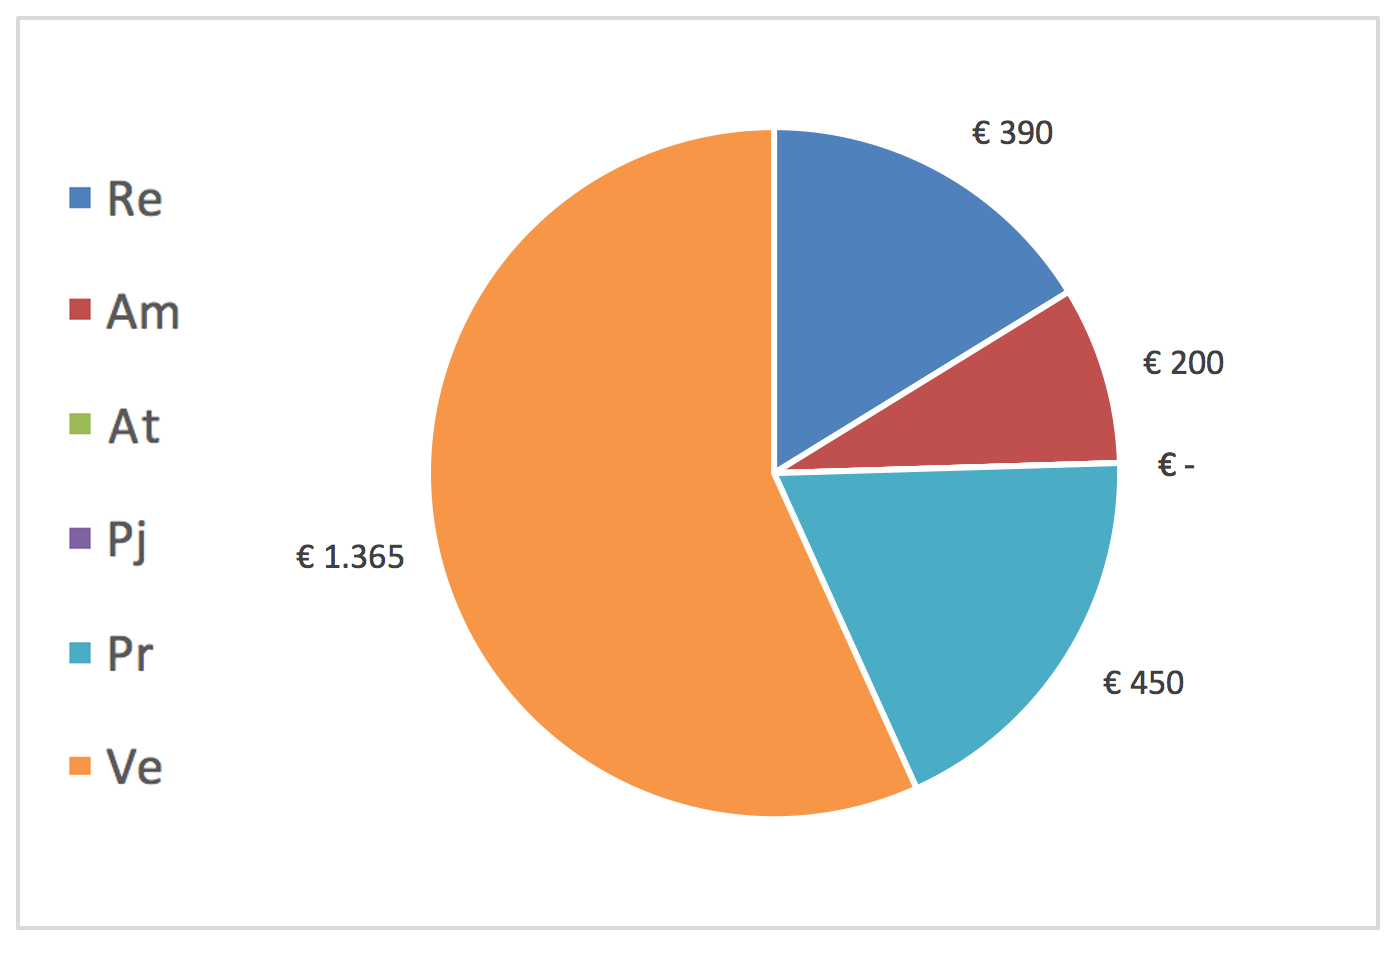
\includegraphics[scale=0.40]{img/s_Totale}
			\caption{Grafico del preventivo economico per ruolo - Totale complessivo}
			\label{fig:Totale complessivo economico}
			\end{figure}
%-----------------------------------------------------------------
		\newpage
		\subsection {Totale rendicontato}
				\subsubsection {Preventivo orario}
                Durante lo sviluppo del progetto, escludendo le ore non rendicontate, i membri del gruppo ricopriranno i vari ruoli secondo la seguente suddivisione:\\
%-----------------------------------------------------------------

							\begin{table}[H] \begin{center} \begin{tabular}{llllllll}
							\toprule
							\textbf{Nominativo}		&	\textbf{Re}	&	\textbf{Am}	&	\textbf{At}	&	\textbf{Pj}	&	\textbf{Pr}	&	\textbf{Ve}	&	\textbf{Tot}\\
							\midrule
							Brutesco	&	5	&	4	&	0	&	26	&	21	&	49	&	105	 \\
							Damo	&	5	&	0	&	0	&	39	&	22	&	39	&	105	 \\
							De Gaspari	&	10	&	10	&	0	&	18	&	25	&	42	&	105	 \\
							Gottardo	&	0	&	6	&	0	&	38	&	28	&	33	&	105	 \\
							Pasqualini	&	13	&	9	&	5	&	45	&	16	&	17	&	105	 \\
							Petenazzi	&	0	&	9	&	5	&	29	&	27	&	35	&	105	 \\
							Prete	&	10	&	0	&	0	&	16	&	32	&	47	&	105	 \\
							\midrule
							Tot in ore	&	43	&	38	&	10	&	211	&	171	&	262	&	735	 \\

							\bottomrule
							\end{tabular} \end{center} \caption{Prospetto orario -
							Totale rendicontato
							}\label{tab:h_TotaleRendicontato} \end{table}		\begin{figure}[H]  \centering  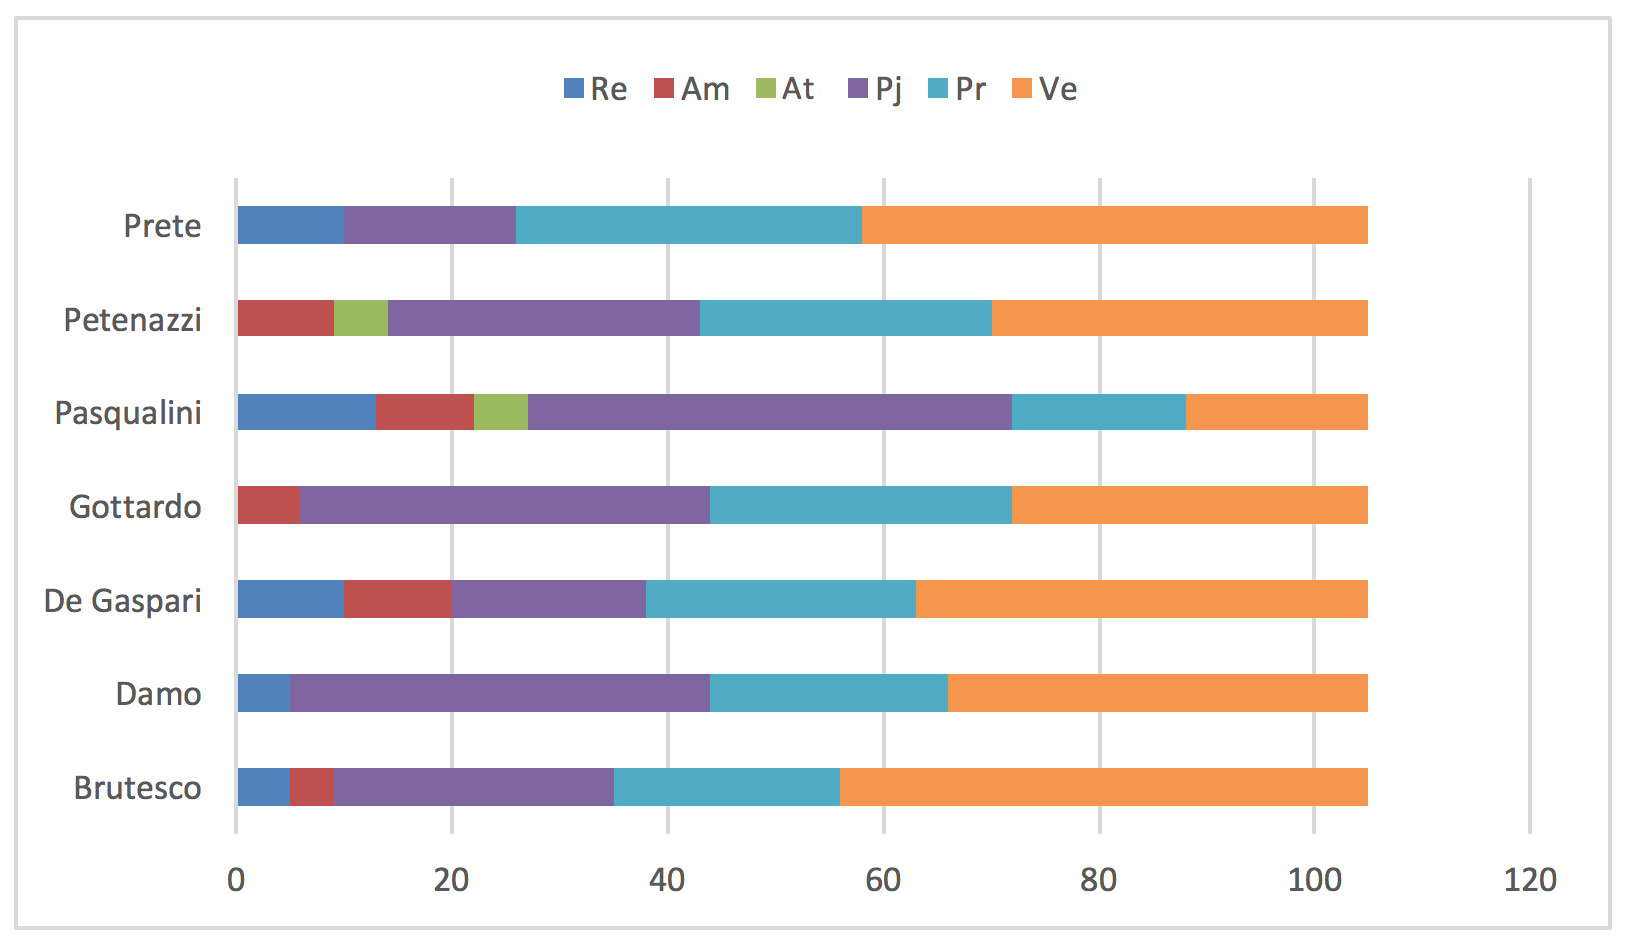
\includegraphics[scale=0.40]{img/h_TotaleRendicontato}
									\caption{Grafico del preventivo orario -								Totale rendicontato	}  \label{fig:h_TotaleRendicontato	} \end{figure}
%-----------------------------------------------------------------
							\begin{figure}[H]
							\centering
							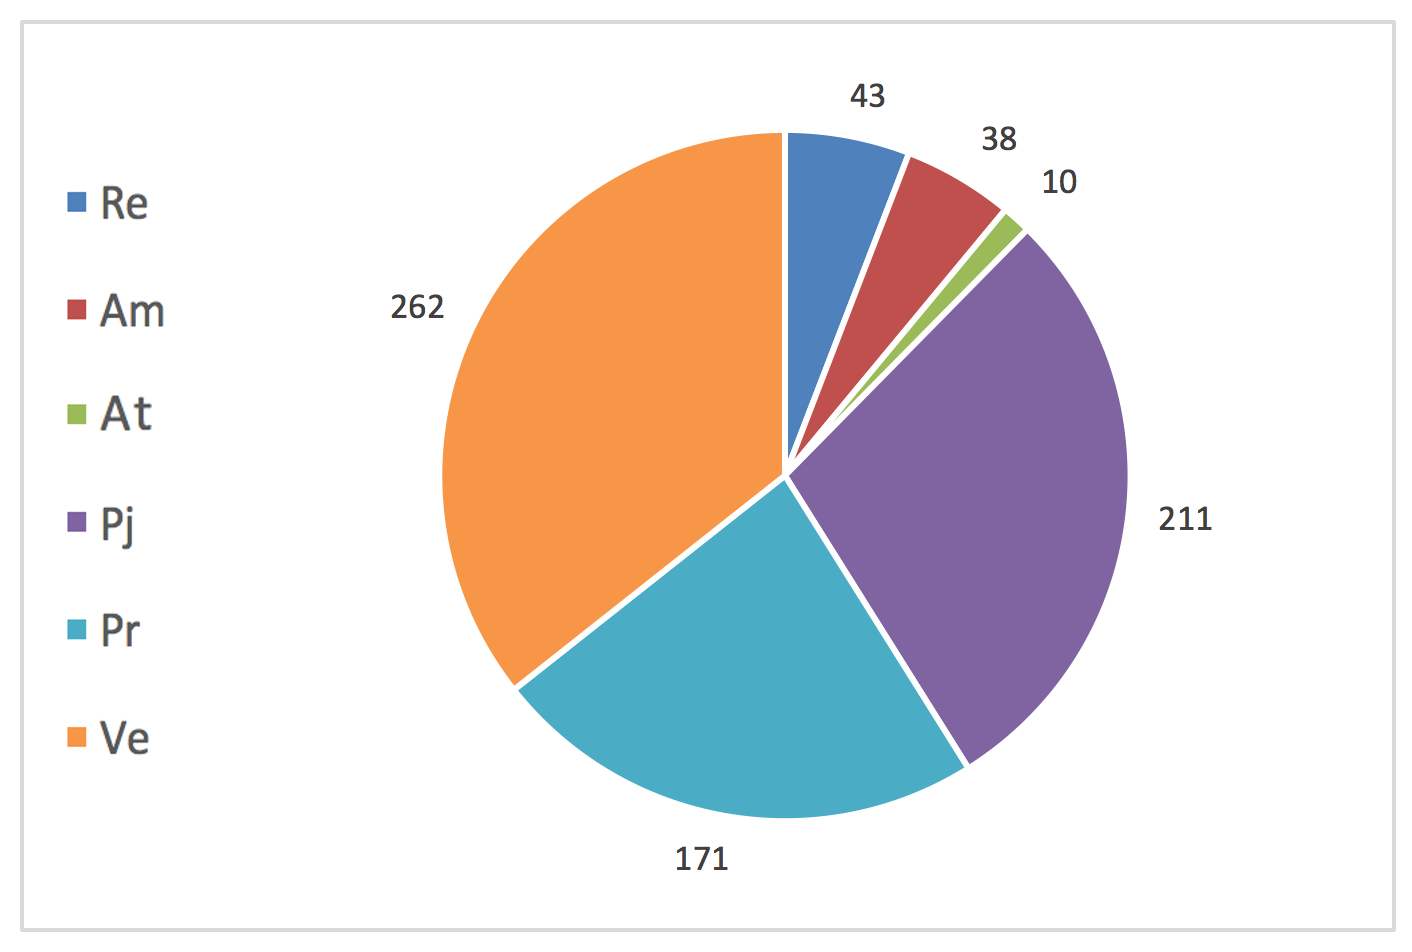
\includegraphics[scale=0.40]{img/h_r_TotaleRendicontato}
							\caption{Grafico del preventivo orario per ruolo - Totale rendicontato}
							\label{fig:Totale rendicontato orario"}
							\end{figure}
%-----------------------------------------------------------------
				\newpage
				\subsubsection {Preventivo economico}
%-----------------------------------------------------------------
							\begin{table}[H] \begin{center} \begin{tabular}{llllllll}
							\toprule
								&	\textbf{Re}	&	\textbf{Am}	&	\textbf{At}	&	\textbf{Pj}	&	\textbf{Pr}	&	\textbf{Ve}	&	\textbf{Tot}\\

							\midrule
							Tot in ore	&	43	&	38	&	10	&	211	&	171	&	262	&	735	 \\


							Tot in €	&	 €  1.290 	 & 	 €      760 	 & 	 €     250 	 & 	 €  4.642 	 & 	 € 2.565 	 & 	 €  3.930 	 & 	 €  13.437 	 \\
							\bottomrule
							\end{tabular} \end{center} \caption{Prospetto economico -
							Totale rendicontato
							}\label{tab:s_TotaleRendicontato} \end{table}
%-----------------------------------------------------------------
%-----------------------------------------------------------------

			\begin{figure}[H]
			\centering
			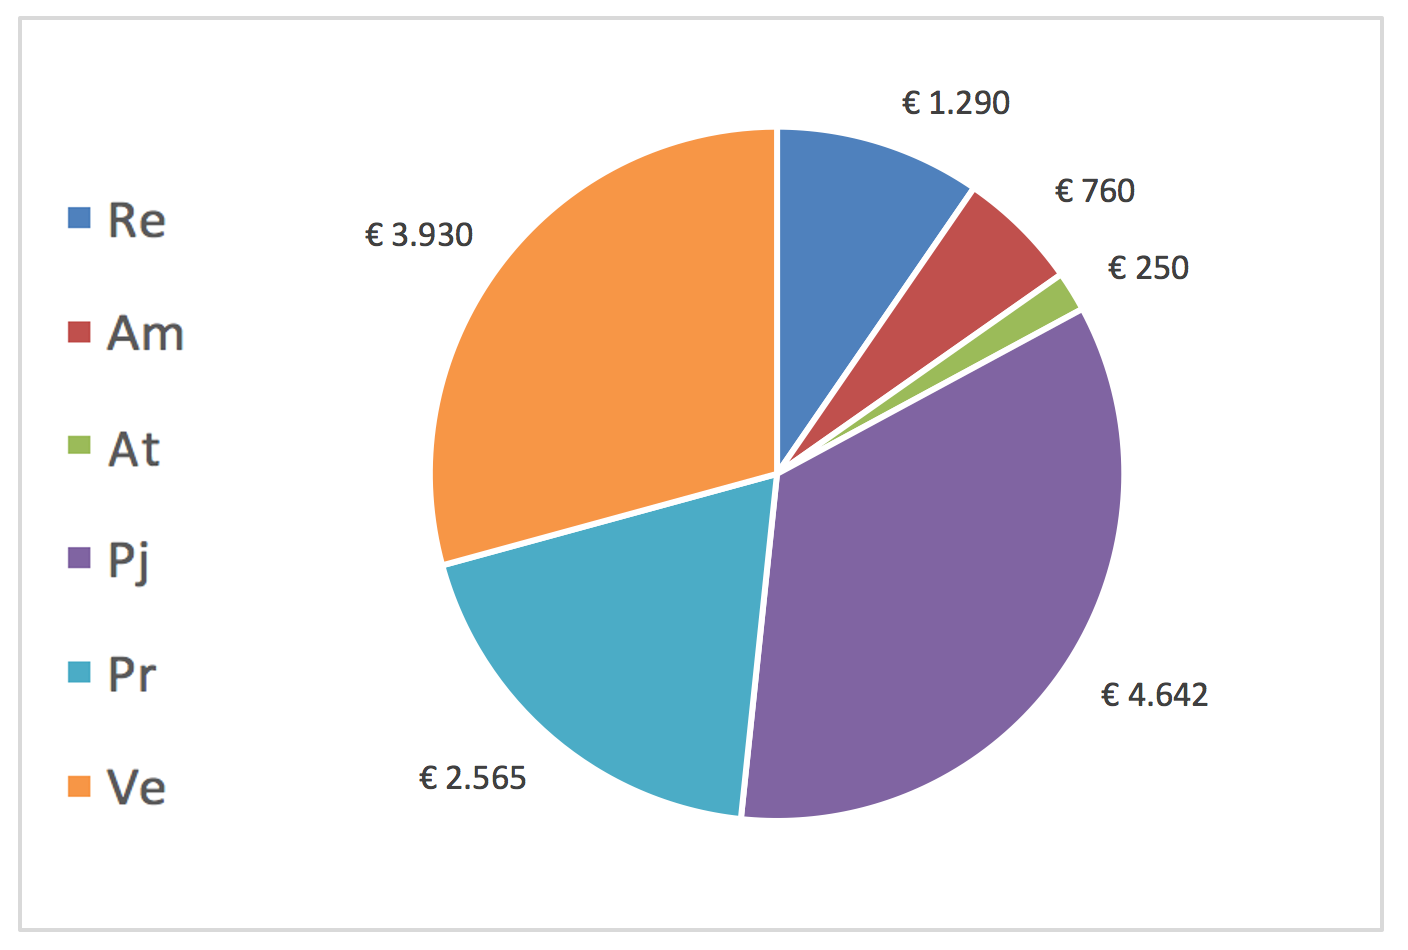
\includegraphics[scale=0.40]{img/s_TotaleRendicontato}
			\caption{Grafico del preventivo economico per ruolo - Totale rendicontato}
			\label{fig:Totale rendicontato economico"}
			\end{figure}
%-----------------------------------------------------------------
\subsection{Costo finale}
Il costo finale del progetto, indicato nella tabella \ref{tab:s_TotaleRendicontato}, viene arrotondato a € 13.430.
